In this chapter, automatic model selection is applied to the problem of nowcasting. It is important to note that while nowcasting may be a fruitful application of automatic model selection, nowcasting (or forecasting) is a fundamentally different problem with a different objective than model selection. While in a stationary world with no breaks the best in-sample model produces the best forecast, this is not the case in a non-stationary world. When dealing with non-stationarity, poor in-sample models can outperform in forecasting, and poor forecasting models can outperform in-sample models.  Therefore this section is included to show an interesting application of Autometrics, the Lasso and BSTS and the results should be interpreted separately from the previous section. 

\section{Google Search Query Data}

The amount of information Google collects through search queries is difficult to comprehend. According Amit Singhal, a Senior Vice President at Google, as of August 2012 Google was processing 100 billion searches every month.\footnote{According to tech blogger Danny Sullivan (2012), this was revealed by Amit Singhal at a press event in San Francisco on August 8th 2012, and is a widely quoted figure.} That means there are over 3.5 billion Google searches each day and over 1 trillion Google searches per year. People turn to Google to get information on just about every aspect of their lives, so it makes sense that Google search queries contain large amounts of information about the state of the world. It is easy to think of cases where Google search queries may contain information about macroeconomic indicators. For example, if an individual loses their job, one of the first places they are likely to go is Google to determine what their unemployment benefits are. Google is also one of the first places they would turn to begin searching for a new job. Thus, Google search queries potentially tell a story about the current state of unemployment in the economy. Similarly, individuals looking to buy new cars are likely to turn to Google to research their options before actually going to a dealership. Google search queries related to new cars could therefore provide insight into current consumer sentiment. Examples of studies which have endeavored to use Google search information for nowcasting and forecasting include D'Amuri and Marcucci (2012), Askitas and Zimmermann (2009) and Webb (2009). 

Google has recently developed several online tools, namely Google Trends and Google Correlate, which allow users to analyze what people have been Googling. Google Trends allows users to enter any search term and see the frequency with which it has been searched over time. Google Correlate allows users to enter a search query and see which other search queries are most correlated with it. Google Correlate has an additional feature which allows the user to enter their own time series and provides the user with the search queries which are most correlated with their submitted time series \cite{WhitePaper}.\footnote{Google Trends is available at \url{https://www.google.co.uk/trends} and Google Correlate is available at \url{https://www.google.com/trends/correlate}.} 

\subsection{Google Flu Trends}

One of the first ways in which the information contained in Google search query data was harnessed was with the Google Flu Trends application. The Center for Disease Control (CDC) in America publishes statistics on the proportion of doctor or hospital visits due to influenza-like illness symptoms (ILI) every week.\footnote{Data is available to download via the FluView Interactive application available at \url{ http://gis.cdc.gov/grasp/fluview/fluportaldashboard.html}} This data is a leading indicator for the prevalence of the flu in the United States. The CDC, however, releases this data at a two-week lag. By economic standards two weeks is not long; most economic statistics are released with at least this much of a lag. For flu epidemics, however, two weeks can be a long time and there can be significant costs to this delay. Action to combat the flu in the form of vaccination, research and public awareness begins later than is ideal. There is therefore obvious value in knowing about a flu outbreak or epidemic as it is beginning. Google developed the Google Flu Trends (GFT) tool with the objective of using Google search queries to accomplish exactly this. GFT produced forecasts - or more precisely nowcasts - using Google search queries to estimate the current measure of ILI. Initially, these nowcasts turned out to be surprisingly accurate.

Google stopped publishing their ILI estimates in 2014, largely because Google Flu Trends performed poorly during the 2013 flu season. While Google never fully disclosed the algorithm behind Google Flu Trends directly, the general approach was outlined in a paper in Nature \cite{naturegoogle}. In this section, Google Flu Trends is revisited, and nowcasts are made using the three algorithms already analyzed. Again, it should be stressed that while in this section automatic model selection algorithms are used to produce nowcasts, model selection itself is a fundamentally different problem, with a different objective, than forecasting or nowcasting. Thus, while nowcasting is an interesting and informative exercise, comparing model selection algorithms for their `model selecting ability' using the accuracy with which they are capable of nowcasting in these sections should be done cautiously, if at all.  
%BSTS, the algorithm analyzed in the previous section, was meant to be an improvement to the original Googel Flu Trends algorithm. 

\section{The Data}

Nowcasting ILI using automatic model selection commences in a similar way to model selection in general. The first step is to formulate the GUM, which includes all variables which may be predictors of ILI at time $t$. An important question then is to consider what data is available at time $t$ which may be relevant for nowcasting ILI. Here, the GUM includes both past ILI values, and relevant Google Correlates, which are explained in this section.

\subsection{Influenza-like-Illness Data}

As mentioned, the CDC releases weekly data on the proportion of GP visits due to influenza-like illness with a two week lag. Weeks are measured from Sunday-Saturday and are numbered either 1-52 or 1-53, depending on how many weeks are in a particular year. Week 1 in a given year is the first week which is entirely in the new year; so Week 1 2016 went from Sunday January 3-Saturday January 9th. New data is published on Fridays and gives the ILI from two weeks earlier. For example, the incidence of ILI for Week 8 2016 which went from Sunday February 21-Saturday February 27 was released on Friday in Week 10 2016 (March 4). This means that if a nowcast for ILI for Week $t$ were to be made on or after Friday of Week $t$, ILI data up to Week $t-2$ is available. Therefore, the GUM can include up until the second lag of ILI. 

\begin{figure}[h]
\centering
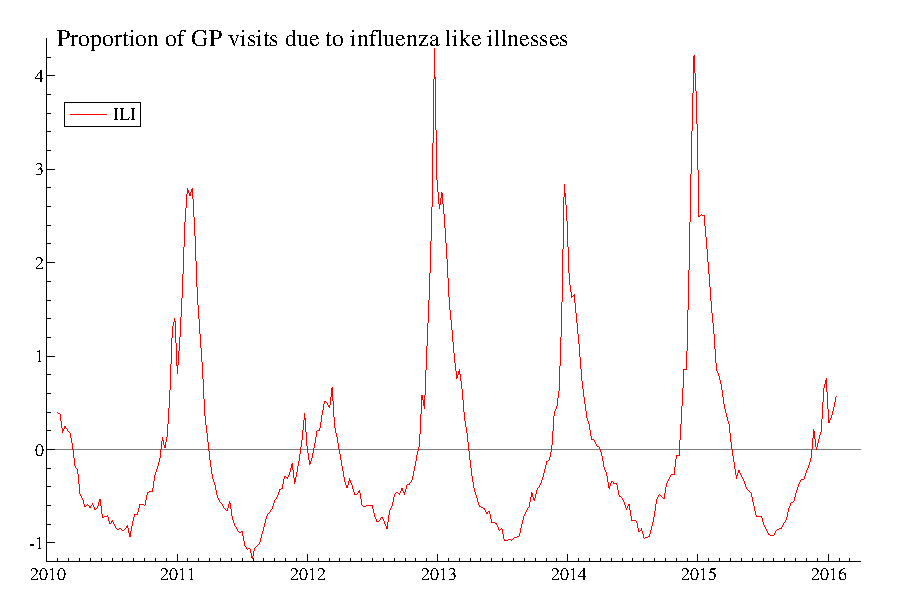
\includegraphics[scale=0.9]{ILIplot}
\caption{Proportion of GP visits due to influenza-like illness}
\label{fig:ILIplot}
\end{figure}



\subsection{Google Correlate Data}

The Google search terms which are most correlated with ILI, called the correlates, as well as their first lags, are also relevant for nowcasting. To find these correlates over a particular period, the weekly ILI time series corresponding to the desired time period was entered into the Google Correlate application. The time period differed with the two different nowcasting approaches taken, which will be explained below. Conveniently, like ILI, Google Correlate measures weeks from Sunday-Saturday. Google Correlate produces a list of the 100 search queries which are most correlated with ILI for the given sample, and also provides the de-meaned and standardized search volume for those 100 search queries as weekly time series. The search volume for a particular query is the proportion of total search queries throughout a given week which were for that query. As a practical matter, Google Correlate data is available to the public with a lag of several weeks. Acknowledging, however, that Google search query data is collected in real time, and in theory would be available for nowcasts, the nowcasting done here assumes that real time data is available. This approach is line with what was done with the original Google Flu Trends tool as well, making the results here comparable. 

\section{Nowcasting with Autometrics, Lasso and BSTS}

Nowcasting here is evaluated using both in-sample and out-of-sample results. In-sample nowcasting refers to a estimating a single model using data from the entire sample period. Fitted values for the sample period are the nowcasts. Out-of-sample nowcasting refers to selecting a holdout period, estimating a model which does not use the data from the holdout period, and using the estimated model to find fitted values for the holdout period. Finding in-sample and out-of-sample nowcasts is relatively straightforward using Autometrics and Lasso. As likely became apparent when the algorithms were described, BSTS is a much more complicated algorithm. Its main purpose, however, is nowcasting and there are features built into the BSTS R package which allow this to be done almost automatically. The reliance of BSTS on Kalman filtering and smoothing, however, means that at this point it is not capable of producing true out-of-sample nowcasts. Therefore, only in-sample nowcasts are results for BSTS.
%At a very basic level, nowcasts are made by drawing from the derived posterior distribution, and taking the mean across these draws. 

\subsection{In-sample Nowcasts using Autometrics and Lasso}
The sample period used to find in-sample nowcasts went from Week 5 2010 to Week 4 2016 (the week beginning January 31 2010 to the week beginning on January 24 2016). The ILI time series was downloaded from the CDC website for this time period, and the observations are denoted $ILI_{1},...,ILI_{313}$ since there are 313 observations in the sample period. The GUM included any variables potentially relevant for modeling ILI. A quick glance at the graph of ILI in Figure \ref{fig:ILIplot} indicates it is likely following an autoregressive process. ILI peaks in the winter around Christmas and is at its lowest in the summer, indicating that seasonality is important. Therefore, lags 2-53 of  ILI were included in the GUM. Admittedly, this is not perfect as the number of weeks in a year varies and, for example, Christmas which likely is relevant to ILI can fall in a different week year-to-year. The other set of regressors in the GUM were the top 100 correlates, and their first lags. These were found by entering the ILI time series for the sample period into the Google Correlate application.  Let $x_{1,t}, x_{2,t},...,x_{100,t}$ denote the search volumes of the top 100 correlates at time $t$. Table \ref{tab:top10correlates} shows the 10 search queries most correlated with ILI for the sample period. To give an example of the correlation structure of the Google correlates, the correlation matrix $\Omega$ of the top ten correlates is:
$$ \Omega = 
\begin{pmatrix}
 1.00  & 0.99  & 0.98  & 0.98  & 0.96  & 0.96  & 0.94  & 0.96  & 0.93  & 0.94 \\
    0.99  & 1.00  & 0.98  & 0.98  & 0.97  & 0.97  & 0.95  & 0.97  & 0.94  & 0.95 \\
    0.98  & 0.98  & 1.00  & 1.00  & 0.96  & 0.96  & 0.94  & 0.95  & 0.93  & 0.94 \\
    0.98  & 0.98  & 1.00  & 1.00  & 0.96  & 0.96  & 0.94  & 0.96  & 0.93  & 0.94 \\
    0.96  & 0.97  & 0.96  & 0.96  & 1.00  & 0.97  & 0.92  & 0.96  & 0.94  & 0.93 \\
    0.96  & 0.97  & 0.96  & 0.96  & 0.97  & 1.00  & 0.93  & 0.96  & 0.95  & 0.93 \\
    0.94  & 0.95  & 0.94  & 0.94  & 0.92  & 0.93  & 1.00  & 0.92  & 0.96  & 0.99 \\
    0.96  & 0.97  & 0.95  & 0.96  & 0.96  & 0.96  & 0.92  & 1.00  & 0.93  & 0.93 \\
    0.93  & 0.94  & 0.93  & 0.93  & 0.94  & 0.95  & 0.96  & 0.93  & 1.00  & 0.95 \\
    0.94  & 0.95  & 0.94  & 0.94  & 0.93  & 0.93  & 0.99  & 0.93  & 0.95  & 1.00 \\

  \end{pmatrix}
$$
\begin{table}
\centering
\begin{tabular}{r|r|r}
\textbf& \textbf{Search query} & \textbf{Correlation with ILI}\\
\hline
$x_{1}$& how to get over the flu & 0.942\\
$x_{2}$&get over the flu	&0.942\\
$x_{3}$&how to get rid of the flu	& 0.932\\
$x_{4}$&get rid of the flu & 0.927	\\
$x_{5}$&flu fever	&0.925\\
$x_{6}$&flu duration	& 0.924\\
$x_{7}$&type a influenza	&0.924\\
$x_{8}$&getting over the flu	&0.919\\
$x_{9}$&tamiflu and pregnancy&	0.918\\
$x_{10}$&influenza type a& 0.917\\
    \end{tabular}%
      \caption{Top 10 correlates and their correlation with ILI}
  \label{tab:top10correlates}%
\end{table}%

The top 100 correlates, their first lags, and the lagged $ILI_{t}$, formed the GUM:
$$ILI_{t}= \alpha + \sum_{i=2}^{53}\gamma_{i}ILI_{t-i}+ \sum_{i=0}^{1}\sum_{j=1}^{100}\beta_{j,i}x_{j,t-i}+u_{t}$$
Autometrics and the Lasso were applied to the above GUM. A significance level $\alpha$ must be selected when using Autometrics, and it is not immediately clear which level should be chosen in this case. This problem is discussed in more detail below, but $\alpha=0.01$ was used. Autometrics returned a model which had 60 parameters selected. Using 10-fold cross validation to select the tuning parameter $\lambda$, Lasso selected a model with 29 parameters. The nowcasts produced by Autometrics and the Lasso are the fitted values, and are plotted against ILI in Figure \ref{ig:InSample}. Table \ref{tab:selvars} displays the mean squared errors, as calculated by:
$$ MSE = \frac{1}{52}\sum_{t=262}^{313}(ILI_{t} - \widehat{ILI_{t}})^{2}$$
where $\widehat{ILI_{t}}$ is the fitted value for ILI at time $t$. Since nowcasts were made for the week of February 1 2015 to the week of January 24 2016, there are 52 nowcasts in total, denoted $\widehat{ILI}_{262},...,\widehat{ILI}_{313}$ to reflect that they correspond to the last 52 observations in the sample. 


\subsection{In-sample Nowcasts using BSTS}
While it is fairly easy to understand how Autometrics and the Lasso calculate their nowcasts, BSTS is more complicated. BSTS deals with time series components and regression components separately, so the first step is determining which time series components, and which regression components to include in the system. Based on the graph of ILI in Figure \ref{fig:ILIplot}, a local linear trend, and seasonal component with $S=53$ are used to model the time series dynamics. The regression component consists of the 100 Google correlates and their first lags, denoted by $\mathbf{x_{t}}$ and $\mathbf{x_{t-1}}$ respectively. Using the state space representation as earlier, ILI can then be described by the following system, which is summarized by `time series + regression components':
\begin{align*}
ILI_{t} &= \mu_{t} + \tau_{t} + \beta_{1}'\mathbf{x_{t}} +\beta_{2}'\mathbf{x_{t-1}} + \epsilon_{t}\\
\mu_{t} &= \mu_{t-1} + \gamma_{t-1} + u_{t}\\
\gamma_{t} &= \gamma_{t-1} + v_{t}\\
\tau_{t} &= - \sum_{s=1}^{52} \tau_{t-s} + w_{t}
\end{align*}
Operationally, BSTS first determines `how much' of $ILI_{t}$ is explained by the local linear trend and seasonality components using Kalman filtering, smoothing and Bayesian data augmentation. Thus, the following system is relevant for the time series component of the algorithm:
\begin{align*}
ILI_{t} &= \mu_{t} + \tau_{t} + \epsilon_{t}\\
\mu_{t} &= \mu_{t-1} + \gamma_{t-1} + u_{t}\\
\gamma_{t} &= \gamma_{t-1} + v_{t}\\
\tau_{t} &= - \sum_{s=1}^{52} \tau_{t-s} + w_{t}
\end{align*}
which is exactly as above, but with the regression component subtracted out. BSTS subtracts the time series component from ILI to end up with $ILI^*$. Then a spike-and-slab regression is used with $ILI^*$ as the dependent variable to determine which of the Google correlates (and their first lags) are relevant for explaining what is not explained by time series components. From the results of the spike-and-slab regression the posterior inclusion probabilities are calculated for each of the Google correlates. Figure \ref{fig:flutrendscomponents} provides a graphical illustration of the contributions of each state. Note that the lines are fuzzy because the draws are graphed. Figure \ref{fig:inclprob} shows Google correlates which have posterior inclusion probability greater than 0.15.

\begin{figure}
\centering
\includegraphics[scale=.8]{bsts-components-flutrends}
\caption{Contributions to ILI by state}
\label{fig:flutrendscomponents}
\end{figure}

\begin{figure}
\centering
\includegraphics[scale=0.5]{bsts-inclusionprob-flutrends}
\caption{Posterior inclusion probabilities for $p>0.15$. White bars indicate the coefficient sign is positive and black bars indicate the coefficient sign is negative.}
\label{fig:inclprob}
\end{figure}


As a Bayesian algorithm, BSTS does not, in fact, calculate fitted values; it derives the predictive posterior distribution for the response variable, and subsequently produces a sample of draws from this distribution \cite{bstspaper}. Nowcasts can then be found by taking the mean across these draws. Figure \ref{ig:InSample} graphs the BSTS nowcasts and Table \ref{tab:selvars} shows the mean squared errors of these nowcasts.
  
\subsection{Comparing In-Sample Nowcasts}

Looking at the graphs in Figure \ref{ig:InSample}, all three algorithms produce reasonably accurate nowcasts. Of the three, the Lasso seems to struggle the most. This is confirmed by the MSEs in Table \ref{tab:selvars}. The number of regressors selected by each of the algorithms, or in the case of BSTS, the number of variables with inclusion probability greater than 0.15, is also shown in Table \ref{tab:selectedvars}. Table \ref{tab:selvars} provides a full list of the variables selected by each algorithm.

Autometrics has the smallest MSE and selects the largest number of variables with 60 of the 252 possible variables selected. BSTS identifies only 10 variables which have posterior inclusion probabilities greater than 0.15. Comparatively, the Lasso's nowcasts are decidedly less accurate. The fact that the Lasso selected half as many variables as Autometrics seems to point to a situation where there is high degree of correlation between the regressors, and where some of these variables are relevant in opposite ways.
The table and graphs show that while all three algorithms are reasonably effective and nowcast with a high degree of accuracy, Autometrics does particularly well. 
%BSTS niter = 4000
\begin{table}
\centering
\begin{tabular}{r|r|r}
 & \textbf{MSE} & \textbf{Variables Selected}\\
 \hline
\textbf{Autometrics} & 0.003 & 60 \\
\textbf{Lasso} & 0.008 & 26\\
\textbf{BSTS} & 0.004 & 10\\
    \end{tabular}%
      \caption{MSEs from in-sample nowcasting}
  \label{tab:selvars}%
\end{table}%



\begin{figure}[h]
\centering
\includegraphics[scale=.95]{All3IS}
\caption{In-sample nowcasts}
\label{ig:InSample}
\end{figure}

% Table generated by Excel2LaTeX from sheet 'compare'
\begin{table}
\small
\singlespacing
  \centering

    \begin{tabular}{l  | l  | l}
    \textbf{BSTS} & \textbf{Lasso} & \textbf{Autometrics} \\
    \hline
    flu type a_1 & anas barbariae & anas barbariae \\
    cough fever& breaking a fever & breaking a fever \\
    get rid of the flu& cold fever & child with flu \\
   home remedies for flue & cough fever & cold fever \\
  cough rememdies  & cough remedies & cold or flu \\
   tamiflu dose & cure a cough & cough fever_1 \\
   flu how long & dangerous fever & cure a cough \\
    is the flu contagious& flu medicines & cure a cough_1 \\
    how to cure the flu& flu medicines_1 & dangerous fever \\
   how long does fever last with flu  & ILI_14 & flu a \\
	 & ILI_15 & flu a_1 \\
    & ILI_16 & flu aches \\
    & ILI_17 & flu aches_1 \\
     & ILI_2 & flu and pregnancy \\
     & ILI_28 & flu how long_1 \\
   & ILI_29 & flu recovery \\
    & ILI_3 & flu remedies_1 \\
     & ILI_50 & flu treatments \\
    & ILI_51 & flu type a \\
     & influenza treatment_1 & flu type a_1 \\
    & tamiflu and breastfeeding & generic tamiflu_1 \\
    & tamiflu drug_1 & get rid of the flu \\
    & tamiflu pediatric dosing & home remedies for flu \\
     & tamiflu side effects & how long contagious \\
     & treat a fever & how long does fever last with flu \\
     & type a flu & how long does it take to get over the flu \\
     &       & how long is the flu contagious \\
     &       & how long is the flu_1 \\
   &       & how to cure the flu \\
     &       & how to cure the flu_1 \\
     &       & how to get rid of flu_1 \\
     &       & how to treat the flu_1 \\
     &       & ILI_2 \\
    &       & ILI_3 \\
          &       & ILI_30 \\
          &       & ILI_4 \\
          &       & ILI_5 \\
          &       & ILI_6 \\
          &       & ILI_9 \\
          &       & influenza a_1 \\
          &       & influenza type a \\
          &       & is the flu contagious \\
          &       & is the flu contagious_1 \\
          &       & medicine for the flu_1 \\
          &       & over the counter flu \\
          &       & remedies for flu_1 \\
          &       & symptoms of pneumonia \\
          &       & tamiflu and alcohol_1 \\
          &       & tamiflu and pregnancy \\
          &       & tamiflu and pregnancy_1 \\
          &       & tamiflu drug_1 \\
          &       & tamiflu side effects \\
          &       & treat a fever \\
          &       & treat a fever_1 \\
          &       & treat the flu \\
          &       & treat the flu_1 \\
          &       & treating the flu_1 \\
          &       & type a flu_1 \\

    \end{tabular}%
      \caption{Selected regressors}
  \label{tab:selectedvars}%
\end{table}%

\subsection{Out-of-sample Nowcasting with Autometrics and the Lasso}

In-sample nowcasting or forecasting where the GUM is the starting point obviously has the potential to be very accurate due to the fact that the training set and the validation set are the same. The example of an extreme case of using OLS when $T=N$, and the fitted values exactly correspond to the true values comes to mind. It is important to consider how nowcasts perform out-of sample, as this reflects the situation in which nowcasts would be made in reality.  A nowcast for time $t$ is based on a model estimated using only the information available at $t$ is a better reflection of how nowcasting would be useful in practice.

To calculate out-of-sample nowcasts using automatic model selection there are several decisions that need to be made. First it must be decided whether the algorithm should reselect a model from the GUM for each successive nowcast. If a new model is estimated for each successive nowcast, another question is whether a rolling or recursive window is more appropriate for determining the sample period. An issue specific to using Google Correlates is whether a new set of correlates should calculated from the Google Flu Trends application for each new nowcast. 

The following explanation is easier to understand with reference to Table \ref{fig:cal}. The chosen sample period went from Week 5 2010 to Week 4 2016 (the week beginning January 31 2010 to the week beginning on January 24 2016) from which there are 313 observations. The `modified holdout' period for which nowcasts were made went from Week 5 2015 and Week 4 2016 (the week beginning February 01, 2015 to the week beginning January 24, 2016). These nowcasts are denoted $\widehat{ILI}_{262},...,\widehat{ILI}_{313}$.  The top 100 Google correlates were found by entering the ILI time series for the sample period excluding the holdout period ($ILI_{1},...,ILI_{261}$) into the Google Correlate application. The top 100 Google correlates are denoted $x_{1,t},...,x_{100,t}$. Variables were selected once and selection was made using only the data in the subsample which excluded the holdout period. So, variables were selected from the following GUM:
$$ILI_{t}= \alpha + \sum_{i=2}^{53}\gamma_{i}ILI_{t-i}+ \sum_{i=0}^{1}\sum_{j=1}^{100}\beta_{j,i}x_{j,t}+u_{t}$$
for $t=1,...,261$. The model estimated from the GUM was used to produce the first nowcast, for the week of Feb 1, 2015, denoted $\widehat{ILI}_{262}$. The reason why the holdout period is `modified' is because for each successive nowcast, an additional observation was added to the sample and a new model was estimated by OLS. The variables included in this model were the variables initially selected by the GUM. Let $z_{1},...,z_{L}$ denote the $L$ regressors selected initially from the GUM. Nowcast $\widehat{ILI}_{262+k}$ was found by estimating the following model, for k=1,..,51:
$$ILI_{t}= \alpha + \sum_{i=1}^{L}\xi_{i}z_{i,t}+ v_{t}, \hspace{1cm} t=1,...,262+k$$
Therefore, new estimates for the $\xi_{i}$s were made to find the new model used to produce each nowcast. The fitted value $\widehat{ILI}_{262+k}$ from the $k^{th}$ model estimated is the nowcast. This process was used for both Autometrics and the Lasso. For Autometrics, the significance level $\alpha$ was set to $0.01$. In the case of Lasso, selecting variables once and using OLS with the selected variables as the regressors for the subsequent nowcasts is equivalent to setting the tuning parameter $\lambda = 0$. The nowcasts and ILI produced by Autometrics and Lasso are graphed in Figure \ref{fig:OutofSample}. The nowcast MSEs, and the number of variables selected by each algorithm is in Table \ref{MSEoutofsample}. Autometrics and Lasso perform similarly, with Lasso achieving a slightly smaller MSE than Autometrics. 
\begin{table}[h]
\centering
\begin{tabular}{r|r|r}
 & \textbf{MSE}& \textbf{Variables Selected} \\
 \hline
\textbf{Autometrics} & 0.016 & 33\\
\textbf{Lasso} & 0.014 & 30 \\
\hline
\textbf{Average} & 0.005 &\\

    \end{tabular}%
      \caption{MSEs from out-of-sample nowcasting}
  \label{MSEoutofsample}%
\end{table}%


The in-sample nowcast graphs indicate that the Autometrics nowcasts tend to be above the true ILI, and that the Lasso's tend to be below the true ILI. A graph of the residuals in Figure \ref{fig:nowcastresiduals} makes this a little clearer. This suggests that perhaps the average of the two nowcasts would produce an even more accurate nowcast. Let $\widehat{ILI}_{ave, t}$ denote this average, $\widehat{ILI}_{auto, t}$ denote the Autometrics nowcast and $\widehat{ILI}_{lasso, t}$ denote the Lasso nowcast as calculcated above. The new average nowcast for time $t$ is:
$$\widehat{ILI}_{ave, t} = \frac{1}{2}(\widehat{ILI}_{auto, t} + \widehat{ILI}_{lasso, t})$$
The average nowcast is also graphed against ILI in Figure \ref{fig:OutofSample}. The MSE of the average is 0.005, which is less than half the MSE of both Autometrics and Lasso individually.  
\afterpage{
\begin{figure}
\includegraphics[scale=.9]{BothPlots}
\caption{Out-of-sample Nowcasts}
\label{fig:OutofSample}
\end{figure}

\begin{figure}
\centering
\includegraphics[scale=.9]{nowcastresiduals}
\caption{Residuals from Autometrics and Lasso nowcasts}
\label{fig:nowcastresiduals}
\end{figure}
}
\afterpage{
\begin{landscape}
\begin{figure}
\centering
\includegraphics{Calendar}
\caption{The timing of in-sample nowcasts and ILI releases}
\label{fig:cal}
\end{figure}
\end{landscape}
}


\subsection{Predicting ILI with Autometrics and the Lasso}

Given that both Autometrics and the Lasso seem reasonably effective at producing accurate nowcasts, an interesting question is whether actual predictions of ILI would be useful. To test this, forecasts of ILI were made using Autometrics and the Lasso.
The forecasting here was done in much the same way as nowcasting was done in the previous section. The sample period from Week 5 2010 to Week 4, 2016 (the week beginning January 31 2010 to the week beginning on January 24 2016) from which there are 313 observations. Forecasts were made for the 52 weeks between Week 5 2015 and Week 4 2016 (the week beginning February 01, 2015 to the week beginning January 24, 2016), and are denoted $\widetilde{ILI}_{262},...,\widetilde{ILI}_{313}$. The top 100 Google correlates were found by entering the $ILI_{t+1}$ time series for the sample period into the Google Correlate application. These correlates, then, are the search terms at time $t$ which are most correlated with ILI at $t+1$ and are denoted $x_{1,t}^{*},...x_{100,t}^{*}$. Again, variables were only selected once, using only the data in the sample period. Thus, the initial model was selected from the GUM:
$$ILI_{t+1}= \alpha + \sum_{i=2}^{53}\gamma_{i}ILI_{t-i}+ \sum_{i=0}^{1}\sum_{j=1}^{100}\beta_{j,i}x_{j,t-i}^{*}+u_{t}$$
The significance level was again set to $\alpha = 0.01$ for Autometrics. The first forecast was made for $ILI_{262}$ and was produced using the model selected from GUM. The fitted value $\widetilde{ILI}_{262}$ from this model is the reported forecast.  For the 51 subsequent forecasts, OLS was used to re-estimate a model using the variables selected by the GUM, and using the information available at the time the forecast was made. For example, the forecast for $ILI_{263}$ was made using information available at $t=262$. If $z_{1},...,z_{L}$ were $L$ the variables selected from the GUM, then to produce $\widetilde{ILI}_{262+k}$, the following model was estimated by OLS:
$$ILI_{t+1}= \alpha + \sum_{i=1}^{L}\xi_{i}z_{i,t}+ v_{t}, \hspace{1cm}  t=1,...,260+k$$
The $k$ fitted values for $ILI_{t+1}$ from each of the $k$ models estimated are the reported forecasts. The forecasts are plotted in Figure \ref{fig:Forecasts}, and the MSEs are reported in Table \ref{tab:MSEforecasts}. The forecasts produced by Autometrics are noticeably less accurate than the nowcasts. The Lasso performs nearly as well at forecasting as it does at nowcasting. The average is better than both, Autometrics and Lasso individually, though only marginally better than the Lasso. 



\begin{figure}[h]
\centering
\includegraphics{forecastplot}
\caption{Forecasts produced by Autometrics, Lasso, and their average.}
\label{fig:Forecasts}
\end{figure}


\begin{table}[h]
\centering
\begin{tabular}{r|rr}
 & \textbf{MSE} &\textbf{Selected Variables} \\
 \hline
\textbf{Autometrics} & 0.032 & 41\\
\textbf{Lasso} & 0.018 & 22 \\
\hline
\textbf{Average} & 0.016 &  \\
    \end{tabular}%
      \caption{MSEs from forecasting}
  \label{tab:MSEforecasts}%
\end{table}%












\subsection{Original Google Flu Trends Estimates}

Since its inception in 2008, the Google Flu Trends model has been updated three times, most recently in 2014. While Google has never released the algorithm it used to compute its ILI estimates, the estimates themselves are available. It has also released the estimates that the revised models produce when applied to historical data.\footnote{ILI estimates from all versions of the Google Flu Trend algorithm can be downloaded from \url{https://www.google.org/flutrends/about/}}. An interesting exercise is then to see how these estimates compare to the estimates produced using the algorithms studied here. 

Figure \ref{fig:2014GFT} graphs the nowcasts produced by Google's 2014 model, for the period January 24, 2010 until October 19 2015 which is the last estimate available.\footnote{The estimates in this graph were downloaded on March 21st from \url{https://www.google.org/flutrends/about/data/flu/historic/us-historic-v3.txt}} Note that it is not clear whether these are in-sample or out-of-sample nowcasts. The nowcast MSE over this period is 0.021, which is larger than the in-sample MSEs for Autometrics, Lasso and BSTS, and the out-of-sample nowcast MSEs produced by Autometrics and the Lasso. 


\begin{figure}
\centering
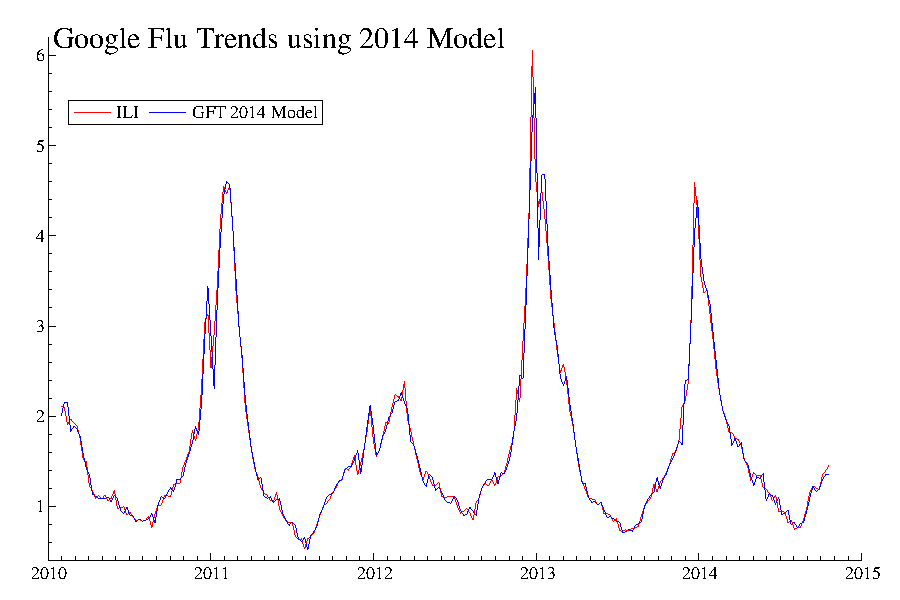
\includegraphics[scale=.8]{GFT2014}
\caption{Nowcasts for 2010-2015 using Google's 2014 model}
\label{fig:2014GFT}
\end{figure}


\section{Selecting the Significance Level for Autometrics}

The accuracy of the nowcasts and forecasts produced by the three different algorithms has been measured by the MSE, which measures how close the predictions and true values are. Clearly, this is a very different way to evaluate the algorithms than the gauge, potency and MSE measures which were used in Chapter 3. When using Autometrics there is strong relationship between the chosen significance level $\alpha$ and the inclusion of irrelevant variables. Approximately $100(\alpha)\%$ of the irrelevant variables present in the GUM are in the model selected by Autometrics. The selection of relevant variables is also influenced by $\alpha$; a higher $\alpha$ means a lower critical value $c_{\alpha}$ which leads to more relevant variables selected. Therefore, when selecting $\alpha$ there exists a tradeoff between setting a low $\alpha$ and excluding most of the irrelevant variables and retaining fewer of the relevant variables, or selecting a high $\alpha$, and retaining most relevant variables, while simultaneously retaining many irrelevant variables. When the goal of using Autometrics is model selection, the consensus is that setting $\alpha$ very low is preferable. However when the goal is not model selection but is instead forecasting, setting a higher $\alpha$ could produce better results. This is due to the fact that in the prediction arena, it is sometimes more costly to exclude relevant variables than it is to retain irrelevant variables. There is a long debate over parsimony versus robustness and it is far from settled, but given that excluding relevant variables is perhaps more costly than including irrelevant variables, it seems sensible to entertain the idea that higher values of $\alpha$ could improve nowcasts and forecasts generated by Autometrics.  
Out-of-sample nowcasts and forecasts were reproduced with this in mind, using the out-of-sample nowcasting and forecasting methods as previously explained, with various values of $\alpha$. The MSE results for the recalculated nowcasts are reported in Table \ref{tab:MSENowcastsdiffalpha}, and results for the recalculated forecasts are reported in Table \ref{tab:MSEForecastdiffalpha}. Averages calculated using the updated nowcasts and forecasts are also reported.  Both the nowcasts and forecasts produced by Autometrics generally improve with the higher levels of significance. 




\begin{table}[h]
\centering

\begin{tabular}{r|r|r|r}
   $\bf{\alpha}$    & \textbf{Autometrics} & \textbf{Average} & \textbf{Variables Selected} \\
  \hline
0.01 &     0.016                                &     0.005           &          33                   \\
0.05 &      0.018                        &     0.005             & 59\\
0.10 &      0.012                                  &    0.008         &62       \\
0.15 &    0.012                                     &     0.005       &   91 \\
0.20&        0.012                              &          0.006     &        92                    
\end{tabular}
\caption{Nowcast MSEs for various levels of $\alpha$}
\label{tab:MSENowcastsdiffalpha}
\end{table}

\begin{table}[h]
\centering

\begin{tabular}{r|r|r|r}
   $\bf{\alpha}$    & \textbf{Autometrics} & \textbf{Average} &\textbf{Variables Selected} \\
  \hline
0.01 &  0.032                         &                0.016            &      41          \\
0.05 &  0.025                         &             0.014     & 48\\
0.10 &     0.015                	    &          0.009         & 73\\
0.15 &   0.017                        &         0.012     & 140\\
0.20 &     0.007      		 &            0.008       &     161                      
\end{tabular}
\caption{Forecast MSEs for various levels of $\alpha$}
\label{tab:MSEForecastdiffalpha}
\end{table}


%\subsection{A Side Note on Bias Correction}

%As explained in Hendry and Krolzig (2005), selection results in biased coefficient estimates. Estimates for relevant variables are biased away from zero since selection depends on $t^{2} > c_{\alpha}^2$. Some relevant variables, particularly if they are `marginally significant' and have low non-centralities, will have $t^2 < c_{\alpha}^2$ and will not be selected. Similarly, some irrelevant variables will be selected as a result $t^2 >c_{\alpha}^2$. This bias can be accounted for using the bias correction method developed by Hendry and Krolzig (2005). Numerous simulation studies have found that bias-correction results in more accurate parameter estimates. 

%Bias correction on the parameters used to produce the nowcasts and forecasts was attempted, however the results turned out to be far less accurate and therefore were not reported.  At first it seemed this could be due to the fact that the bias-correcting mechanism is meant to be used when the variables are orthogonal, and the Google correlates exhibit a high degree of correlation. To account for this, the principal components of the Google Correlates were found. While the bias corrected MSEs improved when using principal components, they were still less accurate than the MSEs where no there was no attempt to bias correct. 

%This is a bit of a puzzle. It could be due to the fact that
%Bias-correction is meant to fix the problem of adventitiously selecting irrelevant variables. In the case of using correlates to predict 

%Higher values of $\alpha$ in Autometrics results in more more variables being selected overall due to a higher critical value and cut-off threshold; this is seen easily with the increasing number of selected variables as $\alpha$ increases in both Table \ref{tab:MSENowcastsdiffalpha} and \ref{tab:MSENowcastsdiffalpha}. To account for this, Hendry and Krolzig (2005) advocate a bias correction mechanism which adjusts parameter estimates downward, to account for the fact that certain irrelevant variables are likely to be included in the selected model. 
%Acknowledging that some irrelevant variables will be adventitiously selected given the higher value of $\alpha$, and considering the high numbers of selected variables, it also seems sensible to employ the bias-correcting mechanism advocated by Hendry and Krolzig (2005),  Since the bias correction mechanism only works in the case of orthogonal variables, and the Google Correlates exhibit a high degree of correlation, the Google Correlates are transformed into their Principal Components.  Due to the high correlation between variables in this setting, it is also necessary to use 


%\subsection{Bias correction}

%As explained in Hendry and Krolzig (2005), selection results in biased coefficient estimates. Estimates for relevant variables are biased away from zero since selection depends on $t^{2} > c_{\alpha}^2$. Some relevant variables, particularly if they are `marginally significant' and have low non-centralities, will have $t^2 < c_{\alpha}^2$ and will not be selected. Similarly, some irrelevant variables will be selected as a result $t^2 >c_{\alpha}^2$. Fortunately, this bias can be accounted for using the bias correction method developed by Hendry and Krolzig (2005). As outlined earlier, the expected t-statistic for a particular variable can be characterized by its non-centrality $\psi$:
%$$ t_{\widehat{\beta}} = \frac{\widehat{\beta}}{\widehat{\sigma_{\beta}}} \simeq \frac{\widehat{\beta}}{\sigma_{\beta}} \sim N[\psi, 1]$$

%Since relevant variables which are selected will be biased away from zero, their t-statistics will be biased in the same direction. This is seen through the expression for the expected t-value of a variable after that variable has been selected. Letting  $\phi(x)$ denote the normal density, and  $\Phi(x)$ denote its integral:

%\begin{align*}
%\psi^* = E[t_{\widetilde{\beta}} |  | t_{\widetilde{\beta}} | > c_{\alpha} ; \psi ] &= \psi + \frac{\phi(c_{\alpha} - \psi) - \phi(-c_{\alpha} - \psi)}{\Phi(c_{\alpha} - \psi) - \Phi(-c_{\alpha} - \psi)}  = \psi + r(\psi, c_{\alpha})\\
%\sigma_{\widetilde{\beta}}E[t_{\widetilde{\beta}} |  | t_{\widetilde{\beta}} | > c_{\alpha} ; \psi ] &= \beta + \sigma_{\widetilde{\beta}}r(\psi, c_{\alpha})\\
%\end{align*}
%since $\beta$ is the unbiased estimator, after estimation an unbiased estimator is given by:
%$$\widetilde{\widetilde{\beta}} = \widetilde{\beta}\frac{\psi}{\psi + r(\psi, c_{\alpha}} $$
%and since
%$$\psi^* = \psi +r(\psi, c_{\alpha})$$
%then (...) add in more steps from Castle et al.
%The bias corrected estimate of $\beta$ is:
%$$ \widetilde\widetilde{\beta} = \widetilde{\beta}\frac{\widetilde{\widetilde{t}}_{\widetilde{\beta}}}{t_{\widetilde{\beta}}}$$


\section{Nowcasting Takeaways}

As this chapter shows, nowcasting is an interesting, relevant and useful application of automatic model selection and depending on the complexity of the algorithm, it can also be employed very easily. As the way that economic data is collected begins to change, and as it starts to become available in real-time, automatic model selection for nowcasting could become a  useful tool for economics, statistical agencies and policy makers alike.  